\documentclass[conference]{IEEEtran}
\usepackage{amsmath,amssymb,graphicx,url}
\title{Rank-Controlled SVD Features for EEG Motor-Imagery Classification Using RBF SVM}
\author{\IEEEauthorblockN{[Student names and USNs]}
\IEEEauthorblockA{[Department and institution]\\Faculty: Dr Geetha KN\\{[Academic year]}}}
\begin{document}
\maketitle
\begin{abstract}
This study evaluates whether low-rank singular value decomposition (SVD) of
electroencephalography (EEG) spectral features improves the accuracy--resource
trade-off for imagined left-versus-right fist classification using a radial basis
function (RBF) support vector machine (SVM). On PhysioNet eegmmidb v1.0.0
(candidate subjects S002--S109; pilot S001 excluded), an automated mechanical
quality audit retained 105 eligible participants (4,723 trials across runs 4, 8,
and 12) and excluded three participants (S088, S092, S100) for 128~Hz sampling.
Fixed 64-channel mu (8--13~Hz) and beta (13--30~Hz) Welch log-bandpower features
(128 dimensions) were standardized and projected using training-only SVD, then
classified with a personalized RBF SVM; a matched RBF SVM without SVD isolated
the projection effect. Hyperparameters were selected per participant via
recording-swapped development validation (runs 4$\leftrightarrow$8) and refitted
on runs 4+8 for a disclosed exploratory follow-up evaluation on run 12 (1,575
trials). On run 12, the no-SVD RBF baseline achieved 56.44\% participant-mean
accuracy (95\% CI [53.67\%, 59.22\%]; macro F1 0.5376), whereas SVD+RBF
achieved 52.63\% (95\% CI [49.94\%, 55.33\%]; macro F1 0.5038) and
training-majority achieved 49.84\% (macro F1 0.3323). Paired participant
differences (SVD minus baseline) were $-3.81$ percentage points in accuracy
(95\% CI [$-6.47$, $-1.14$]~pp) and $-0.0337$ in macro F1 (95\% CI [$-0.0621$,
$-0.0053$]). Neither pipeline reached the 75\% aspiration target. Although SVD
reduced total serialized pipeline storage by 61.5\% (1.39~MB vs.\ 3.61~MB across
105 models), Welch bandpower extraction (~16~ms/batch) dominated end-to-end
feature-plus-classifier runtime (~17~ms/batch for both methods), yielding
negligible inference speedup. Unsupervised variance-preserving SVD therefore
traded classification accuracy for model compactness under this small-sample
personalized protocol.
\end{abstract}
\begin{IEEEkeywords}
EEG, motor imagery, singular value decomposition, support vector machine, RBF kernel
\end{IEEEkeywords}

\section{Introduction}
Motor imagery can modulate sensorimotor EEG rhythms without overt movement.
Event-related synchronization and desynchronization (ERS/ERD) in the mu
(8--13~Hz) and beta (13--30~Hz) bands motivate spectral features, but scalp EEG
has low signal-to-noise ratio and substantial inter-subject and inter-recording
variability~\cite{ref3}. PhysioNet's EEG Motor Movement/Imagery dataset
(eegmmidb v1.0.0) provides 64-channel recordings acquired with BCI2000~\cite{ref1}.
The task studied here is binary classification of imagined left versus right fist
movement from runs 4, 8, and 12.

When each participant has only two short development recordings (~30 trials
combined) and 128 spectral features, dimensionality reduction is a natural
candidate for controlling model complexity and storage. The project-specific
research question is whether rank-controlled linear SVD of standardized bandpower
features offers a favorable classification--resource trade-off compared with an
identical RBF SVM without SVD when training and evaluation recordings are kept
strictly separate. This is an empirical trade-off study rather than a claim that
SVD--SVM is a novel algorithm. Our contributions are: (1) a self-contained,
leakage-guarded personalized SVD+RBF pipeline with automated mechanical auditing
and SHA-256 provenance; (2) a strictly matched no-SVD ablation using identical
features, splits, and SVM grid; and (3) a full-cohort (105-participant)
evaluation reporting classification metrics, participant-level confidence
intervals, paired differences, reconstruction diagnostics, separated stage
timings, and per-model and aggregate storage.

\section{Mathematical Background}
\subsection{Spectral representation}
Each post-cue trial is a matrix $X_i\in\mathbb{R}^{64\times 320}$ in volts
(64 channels over 2~s at 160~Hz). Welch averaging estimates the power spectral
density $\widehat S_{ic}(f)$~\cite{ref13} per channel $c$. Integrating over the
mu ($B_1=[8,13]$~Hz) and beta ($B_2=[13,30]$~Hz) bands via the trapezoidal rule
and applying a floored base-10 logarithm yields
\begin{equation}
F_{i,(b,c)}=\log_{10}\!\left(\max\left\{\int_{B_b}\widehat S_{ic}(f)\,df,\;\epsilon\right\}\right),
\end{equation}
with $\epsilon=10^{-20}\;\text{V}^2$, producing $d=128$ features per trial.
Training-fold means $\mu_j$ and standard deviations $s_j$ yield standardized
features $A_{ij}=(F_{ij}-\mu_j)/s_j$; validation and test recordings are
transformed using those same training statistics.

\subsection{Singular Value Decomposition (SVD)}
For the standardized training matrix $A\in\mathbb{R}^{N_{\text{train}}\times 128}$,
the thin SVD~\cite{ref10,ref11,ref12} is
\begin{equation}
A=U\Sigma V^T,\qquad Z=AV_r,\qquad \widehat A=AV_rV_r^T,
\end{equation}
where $V_r\in\mathbb{R}^{128\times r}$ holds the leading $r$ right singular
vectors corresponding to the largest singular values $\sigma_1\ge\cdots\ge\sigma_r$.
Any unseen standardized trial row $a\in\mathbb{R}^{1\times 128}$ is projected as
$z=aV_r\in\mathbb{R}^{1\times r}$ using only the training-fitted basis $V_r$,
never rows of $U$.

\subsection{RBF Kernel SVM}
With labels $y_i\in\{-1,+1\}$, the soft-margin SVM solves~\cite{ref7,ref8}
\begin{equation}
\min_{w,b,\xi\geq 0}\;\tfrac12\|w\|^2+C\sum_{i=1}^{N_{\text{train}}}\xi_i
\quad\text{s.t.}\quad y_i(w^T\phi(z_i)+b)\geq 1-\xi_i.
\end{equation}
Using the Gaussian RBF kernel $K(z,z')=\exp(-\gamma\|z-z'\|^2)$, the decision
function is $\operatorname{sign}\!\left(\sum_i\alpha_i y_i K(z_i,z)+b\right)$,
where nonzero dual coefficients $\alpha_i\in(0,C]$ identify support vectors.
Regularization $C>0$ penalizes margin violations and $\gamma>0$ controls kernel
locality.

\section{Existing Methods}
Supervised spatial filtering, particularly Common Spatial Patterns (CSP), is a
widely used EEG motor-imagery method~\cite{ref4,ref5}, extended across multiple
sub-bands by Filter-Bank CSP (FBCSP)~\cite{ref6}. Kernel PCA~\cite{ref9} performs
nonlinear feature extraction, whereas our SVD projection is strictly linear and
only the downstream SVM uses an RBF kernel. End-to-end convolutional networks
such as Dose et al.~\cite{ref14} and EEGNet~\cite{ref15} learn spatiotemporal
filters directly from EEG but lie outside our scope. MNE-Python supports
reproducible EEG preprocessing~\cite{ref2}, and MOABB motivates standardized BCI
benchmarking~\cite{ref16}. Our accompanying survey documents 16 DOI-verified
references separating mathematical foundations from EEG-specific studies; we do
not claim exhaustive literature coverage or algorithmic novelty.

\section{Proposed Method}
The implemented workflow enforces strict separation of auditing, development
selection, follow-up evaluation, and reporting:
\begin{enumerate}
\item Audit candidate EDF files (S002--S109) using objective mechanical checks
  and record SHA-256 file hashes.
\item Filter each run independently (8--30~Hz zero-phase FIR), epoch $[0.5,2.5)$~s
  post cue, and compute deterministic 128-D Welch log-bandpower features.
\item Within each development fold (run 4$\to$8 and run 8$\to$4), fit a fresh
  \texttt{StandardScaler}, \texttt{SVDProjector} (for SVD+RBF), and RBF
  \texttt{SVC} on the training run only.
\item Select per-participant $(r,C,\gamma)$ for SVD+RBF and $(C,\gamma)$ for
  the no-SVD baseline by mean development macro F1 with deterministic tie-breaking.
\item Lock selections with SHA-256 digests; refit both pipelines on combined
  development runs 4+8.
\item Evaluate run 12 once per locked selection for every eligible participant,
  alongside a development-trained majority-class baseline.
\end{enumerate}

\section{Mathematical Analysis}
By the Eckart--Young theorem~\cite{ref11}, truncated SVD minimizes the relative
Frobenius reconstruction error of the standardized training feature matrix:
\begin{equation}
E_r=\frac{\|A-\widehat A\|_F}{\|A\|_F}
=\sqrt{\frac{\sum_{j>r}\sigma_j^2}{\sum_j\sigma_j^2}},
\end{equation}
with retained training spectral energy $1-E_r^2$. Crucially, this optimizes
unsupervised variance reconstruction of bandpower, not class separability; a
low-variance singular direction can still carry left-versus-right discriminative
information. Because training features are centered by \texttt{StandardScaler},
the numerical rank of $A$ is at most $\min(N_{\text{train}}-1,128)$ ($\le 14$
for a 15-trial development fold and $\le 29$ for a 30-trial refit).

Computationally, projection costs $O(128r)$ multiply-adds per trial and stores
$128r$ floating-point basis entries. RBF SVM prediction scales as $O(n_{\text{SV}}r)$
rather than $O(n_{\text{SV}}\cdot 128)$, where $n_{\text{SV}}$ is the support
vector count. However, end-to-end inference also includes Welch PSD computation,
so classifier-only speedups need not translate into total latency reductions.
Likewise, deployed model storage must account for the scaler, basis $V_r$, and
support-vector arrays summed across all personalized models.

\section{Experimental Design}
\subsection{Dataset, audit, and preprocessing}
Candidate participants were S002--S109 from PhysioNet eegmmidb v1.0.0; Subject~1
was prespecified as an excluded pilot. Eligibility required readable runs 4, 8,
and 12, 64 consistently ordered standard 10--05 EEG channels, 160~Hz sampling,
only T0/T1/T2 annotations with both T1 (left, label~0) and T2 (right, label~1)
present (T0 excluded), and finite non-overlapping in-bounds epochs. Each run was
independently bandpass-filtered (8--30~Hz, zero-phase FIR \texttt{firwin}),
epoched on $[0.5,2.5)$~s post cue ($64\times 320$ samples), and transformed via
Welch PSD (Hann window, 160-sample segments, 80-sample overlap, constant
detrend, density scaling) integrated on $[8,13]$ and $[13,30]$~Hz with a
$10^{-20}\;\text{V}^2$ floor in \texttt{float64}. Fig.~\ref{fig:eeg} shows an
illustrative raw versus filtered trace and single trials from eligible Subject~2.

\begin{figure}[ht]
\centering
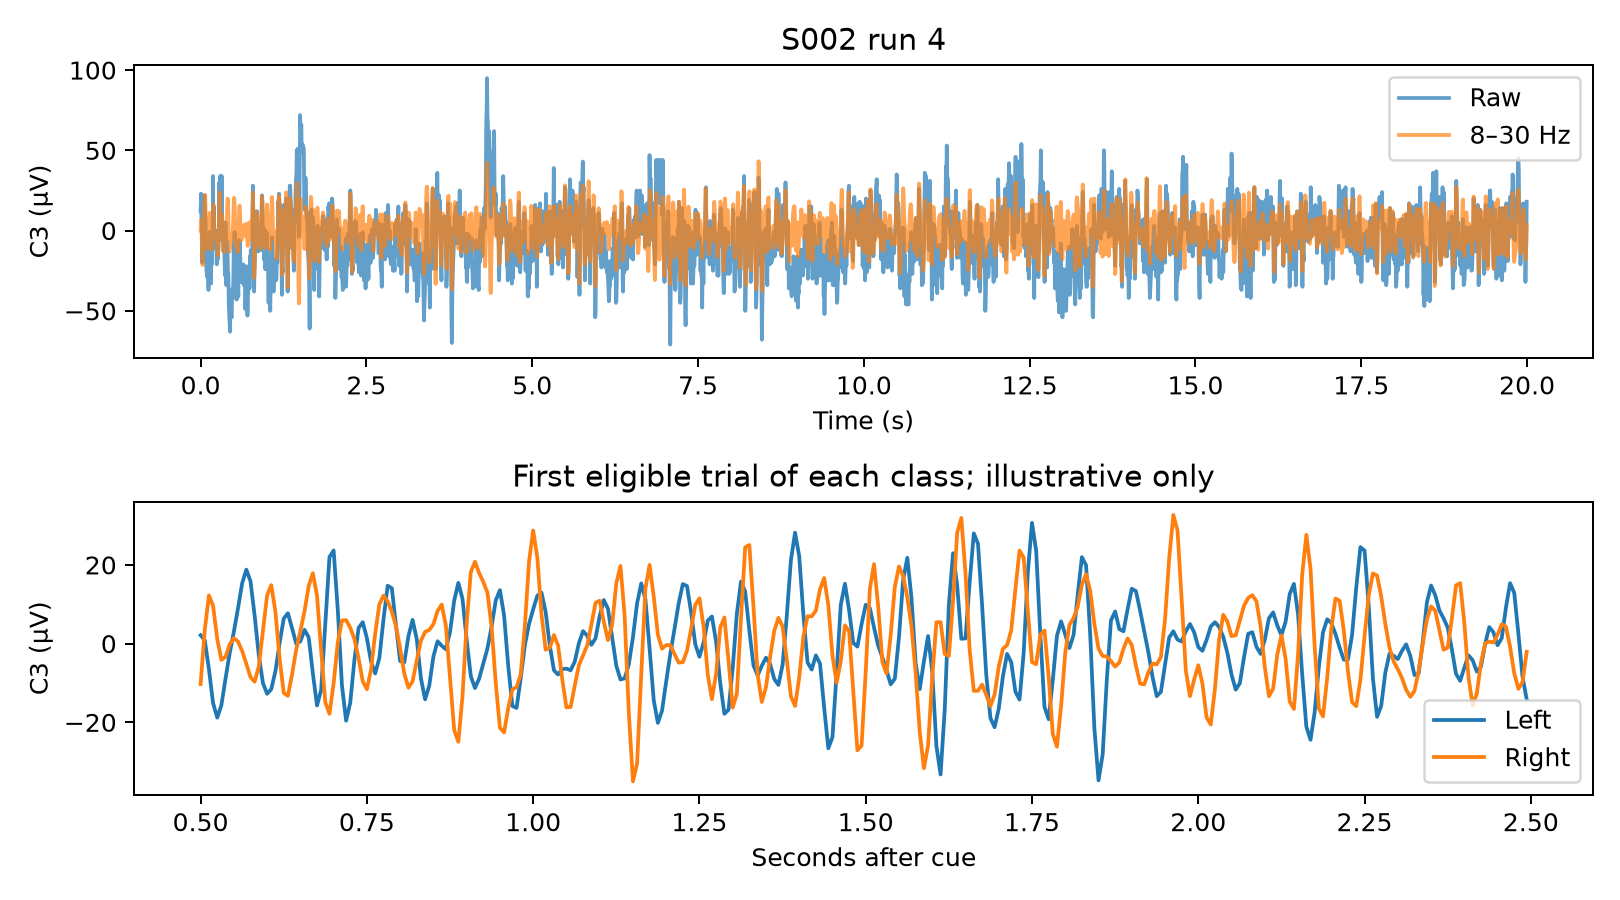
\includegraphics[width=\columnwidth]{../figures/eeg_example.png}
\caption{Illustrative C3 channel trace (raw vs.\ 8--30~Hz FIR filtered) and
first left/right filtered trials from eligible participant S002, run~4.}
\label{fig:eeg}
\end{figure}

\subsection{Validation, locking, and prior exposure disclosure}
Development validation swapped complete runs 4 and 8 per participant. Candidate
SVD ranks $r\in\{2,4,6,8,10,12\}$ were bounded by the minimum training-fold
numerical rank; both pipelines searched $C\in\{0.1,1,10,100\}$ and
$\gamma\in\{\text{scale},0.001,0.01,0.1\}$ (96 candidates for SVD+RBF vs.\ 16
for the no-SVD baseline). Selection prioritized mean development macro F1, then
balanced accuracy, smaller rank, smaller $C$, and fixed $\gamma$ order.

\textbf{Prior exposure disclosure:} Run~12 outcomes on this cohort were
inspected in earlier work. Accordingly, the present run~12 evaluation is an
\emph{exploratory follow-up evaluation}, not a fresh untouched confirmatory
test. Hyperparameters were locked solely from runs 4 and 8 and were never
revised using run~12. All experiments ran on Windows~11 (AMD64, 16 logical
CPUs) with Python~3.13.6, NumPy~2.5.5, SciPy~1.18.1, scikit-learn~1.9.1,
MNE~1.13.2, pandas~3.1.1, and joblib~1.6.0.

\section{Results}
\subsection{Cohort audit and development selection}
Of 108 candidates (S002--S109), \textbf{105 participants were eligible} and
\textbf{3 were excluded} objectively for 128~Hz sampling (\texttt{sfreq\_mismatch: 128.0}:
S088, S092, S100). Across the 315 eligible recordings, 4,723 trials were
extracted (2,383 left, 2,340 right): 1,575 in run~4 (797 left, 778 right),
1,573 in run~8 (792 left, 781 right), and 1,575 in run~12 (794 left, 781 right).

During runs 4$\leftrightarrow$8 development validation, SVD+RBF attained higher
mean development macro F1 (0.6267) than the no-SVD baseline (0.5406). Selected
SVD ranks spanned the full grid: $r=2$ (37 participants), $r=4$ (17), $r=6$
(13), $r=8$ (14), $r=10$ (10), and $r=12$ (14), with mean rank 5.71 (median 4)
and mean feature-dimension reduction 35.15$\times$ (range 10.67$\times$--64.00$\times$).

\subsection{Exploratory run 12 classification performance}
Table~\ref{tab:results} and Fig.~\ref{fig:acc} summarize run~12 performance
across all 105 eligible participants (1,575 test trials). On participant-averaged
metrics, the no-SVD RBF baseline achieved \textbf{56.44\%} accuracy (SD 14.35\%,
95\% $t$-CI [53.67\%, 59.22\%]), 56.47\% balanced accuracy (95\% CI [53.71\%,
59.23\%]), and \textbf{0.5376} macro F1 (95\% CI [0.5075, 0.5676]; macro
precision 0.5711, macro recall 0.5647). SVD+RBF achieved \textbf{52.63\%}
accuracy (SD 13.93\%, 95\% CI [49.94\%, 55.33\%]), 52.69\% balanced accuracy
(95\% CI [50.01\%, 55.36\%]), and \textbf{0.5038} macro F1 (95\% CI [0.4752,
0.5324]; macro precision 0.5240, macro recall 0.5269). The training-majority
baseline achieved 49.84\% accuracy (95\% CI [49.19\%, 50.49\%]), 50.00\%
balanced accuracy, and 0.3323 macro F1.

Pooled across all 1,575 run~12 trials, accuracy matched the participant means
(56.44\% baseline vs.\ 52.63\% SVD+RBF; pooled macro F1 0.5636 vs.\ 0.5257;
Fig.~\ref{fig:cm}). Neither method achieved the 75\% aspiration target at the
cohort level: only 5/105 baseline participants (range 13.33\%--86.67\%, median
60.00\%) and 6/105 SVD+RBF participants (range 20.00\%--86.67\%, median 53.33\%)
reached $\ge$75\% accuracy on their 15-trial run~12 test set.

\begin{table}[ht]
\centering
\caption{Exploratory run~12 evaluation across all 105 eligible participants (1,575 trials).}
\label{tab:results}
\begin{tabular}{lcccc}\hline
Method & Acc.\ (\%) & Bal.\ Acc.\ (\%) & Macro F1 & Storage (MB) \\ \hline
RBF without SVD & 56.44 & 56.47 & 0.5376 & 3.61 \\
SVD + RBF & 52.63 & 52.69 & 0.5038 & 1.39 \\
Training-majority & 49.84 & 50.00 & 0.3323 & 0.00 \\
\hline\end{tabular}
\end{table}

\begin{figure}[ht]
\centering
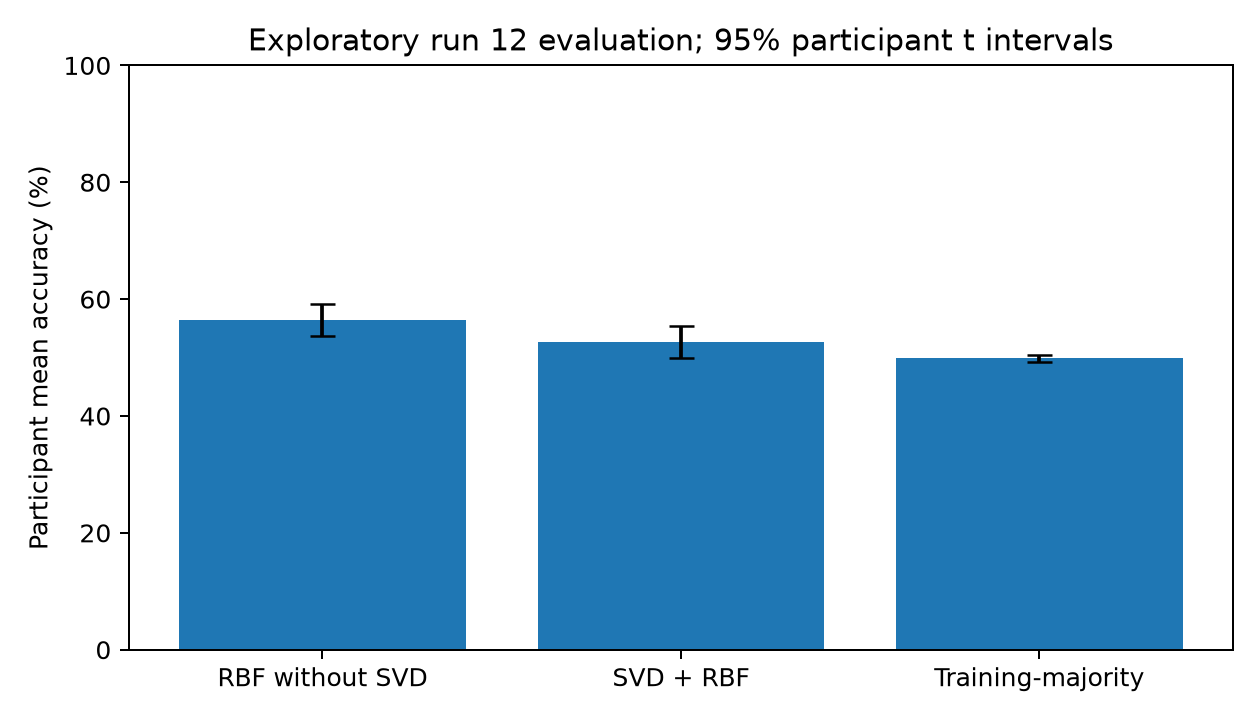
\includegraphics[width=\columnwidth]{../figures/accuracy.png}
\caption{Participant-mean run~12 accuracy with 95\% participant $t$-intervals ($N=105$).}
\label{fig:acc}
\end{figure}

\begin{figure}[ht]
\centering
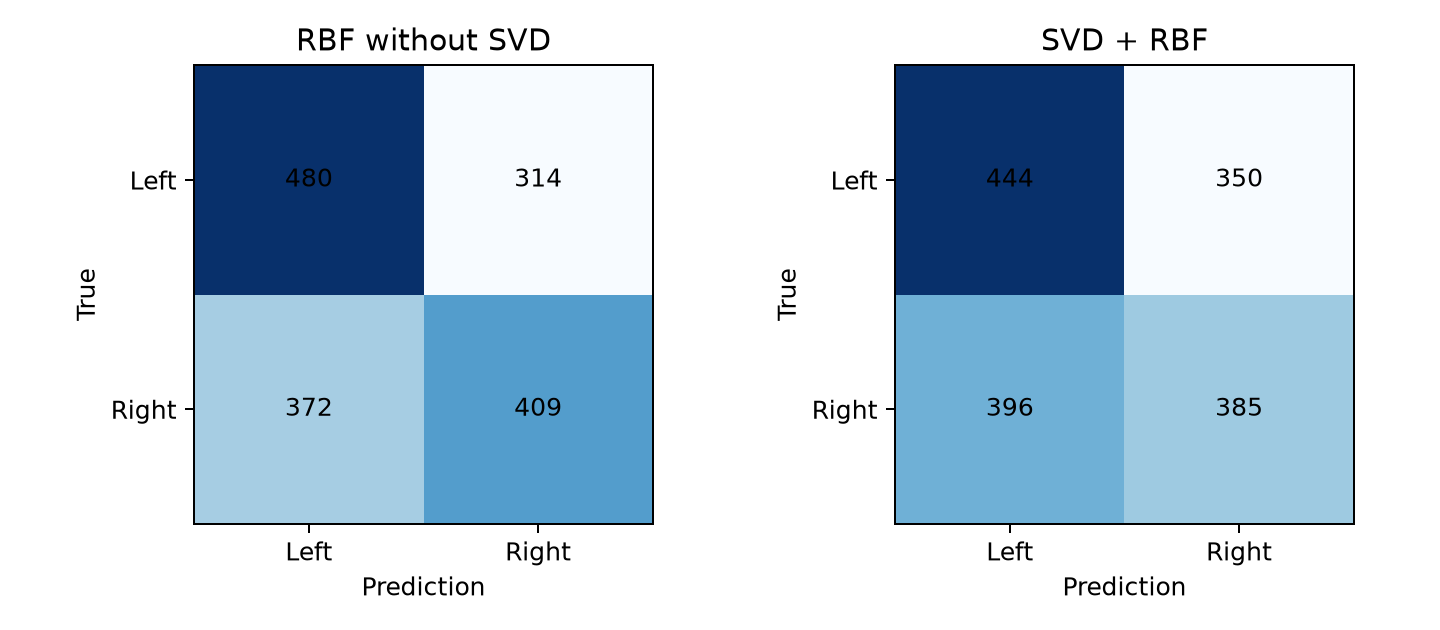
\includegraphics[width=\columnwidth]{../figures/confusion_matrices.png}
\caption{Pooled run~12 confusion matrices (1,575 trials: 794 left, 781 right) for
RBF without SVD (left) and SVD+RBF (right).}
\label{fig:cm}
\end{figure}

\subsection{SVD spectral energy and reconstruction diagnostics}
Refitted on combined development runs 4+8, the selected SVD bases retained a
mean of 78.27\% of standardized training spectral energy (SD 12.47\%, range
46.94\%--95.40\%). Relative Frobenius reconstruction error of standardized
bandpower averaged 0.4462 on runs 4+8 (SD 0.1357, range 0.2145--0.7284) and rose
to 0.5634 on unseen run~12 (SD 0.1094, range 0.3202--0.8229; Fig.~\ref{fig:svd}),
reflecting inter-recording distribution shift.

\begin{figure}[ht]
\centering
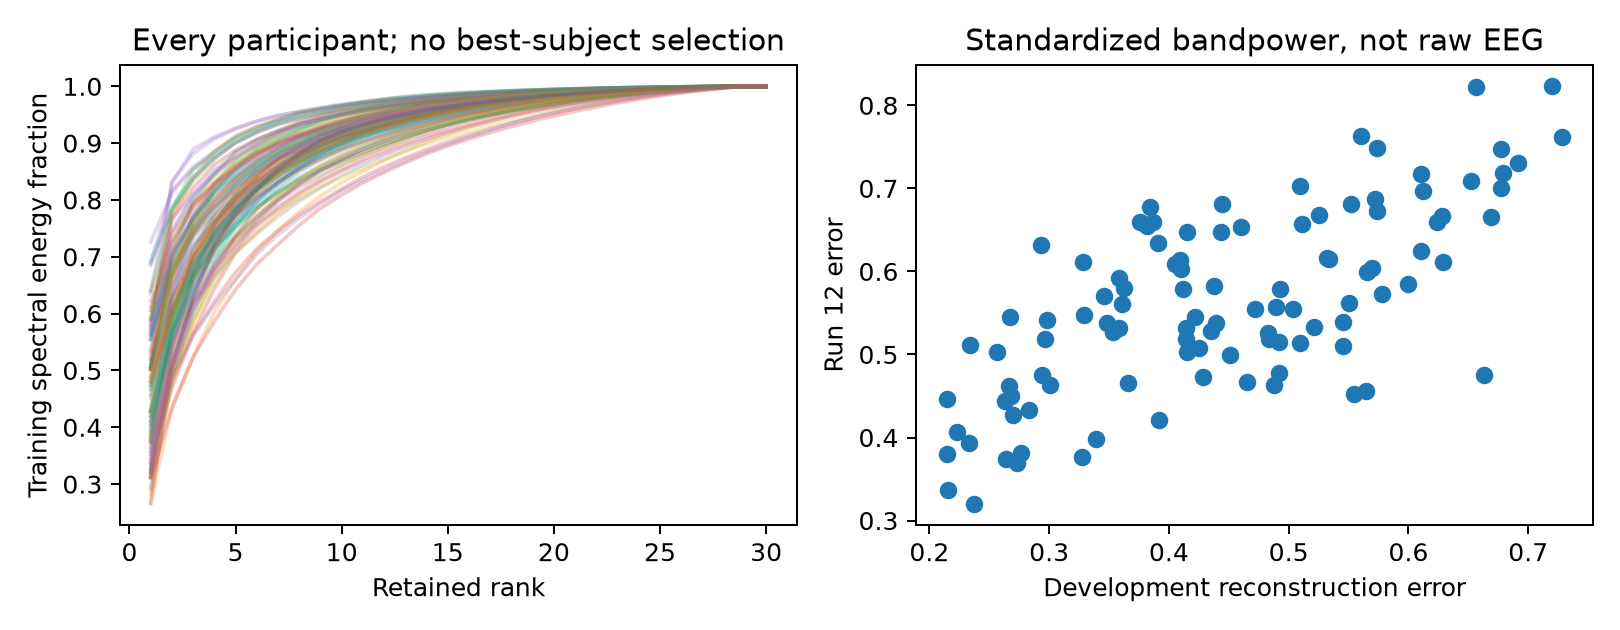
\includegraphics[width=\columnwidth]{../figures/svd_diagnostics.png}
\caption{Cumulative training spectral energy across all 105 participants (left)
and development vs.\ run~12 standardized bandpower reconstruction error (right).}
\label{fig:svd}
\end{figure}

\section{Comparison}
\subsection{Paired classification comparison}
Pairing each participant's SVD+RBF and no-SVD baseline scores ($N=105$) shows a
consistent accuracy drop from SVD compression: mean paired difference (SVD minus
baseline) was \textbf{$-3.81$~pp} in accuracy (SD 13.77~pp, 95\% CI [$-6.47$,
$-1.14$]~pp), \textbf{$-3.78$~pp} in balanced accuracy (95\% CI [$-6.41$,
$-1.16$]~pp), and \textbf{$-0.0337$} in macro F1 (95\% CI [$-0.0621$,
$-0.0053$]). SVD outperformed the baseline for 27 participants, tied for 28,
and underperformed for 50. Notably, although SVD+RBF scored higher during
development validation (0.6267 vs.\ 0.5406 macro F1), searching 6$\times$ more
hyperparameter combinations (96 vs.\ 16) over only ~15 trials per fold induced
greater selection optimism that did not generalize to run~12.

\subsection{Runtime and storage trade-offs}
Table~\ref{tab:resources} separates fixed I/O and preprocessing from repeated
warm feature-plus-classifier timings (5 repeats per participant on the 15-trial
run~12 batch). Fixed run~12 EDF loading (median 22.48~ms) and 8--30~Hz FIR
filtering plus epoching (median 112.98~ms) dominate offline preparation. Within
the warm inference path, classifier-only \texttt{svm.predict} was slightly
faster with SVD (median 0.34~ms vs.\ 0.39~ms), whereas representation transform
was slightly slower (0.81~ms vs.\ 0.62~ms) and Welch bandpower extraction
(15.80--16.00~ms) accounted for over 93\% of total feature-plus-classifier batch
time (~16.92~ms vs.\ ~16.99~ms, or 1.13~ms/trial amortized throughput, which is
not measured single-trial real-time latency). Representation fitting took longer
with SVD (2.17~ms vs.\ 1.21~ms).

In contrast, storage showed a clear reduction: mean per-participant serialized
joblib pipeline size fell from 34,403~B (range 28,173--36,541~B) to 13,240~B
(range 8,397--21,485~B), reducing total cohort storage across 105 personalized
models by \textbf{61.5\%} (3,612,293~B vs.\ 1,390,149~B; parameter-array
estimates 3.39~MB vs.\ 1.15~MB).

\begin{table}[ht]
\centering
\caption{Median per-participant stage timings (ms, 15-trial run~12 batch; 5 warm repeats) and cohort storage ($N=105$).}
\label{tab:resources}
\begin{tabular}{lcc}\hline
Measure & RBF without SVD & SVD + RBF \\ \hline
Representation fit (ms) & 1.21 & 2.17 \\
SVM fit (ms) & 1.37 & 1.44 \\
Welch bandpower (ms) & 16.00 & 15.80 \\
Representation transform (ms) & 0.62 & 0.81 \\
Classifier-only predict (ms) & 0.39 & 0.34 \\
Feature + classifier batch (ms) & 16.99 & 16.92 \\
Amortized throughput (ms/trial) & 1.13 & 1.13 \\
Mean serialized pipeline (B) & 34,403 & 13,240 \\
Total 105-model storage (B) & 3,612,293 & 1,390,149 \\
\hline\end{tabular}
\end{table}

\section{Limitations}
First, with only ~15 trials per recording and two development folds,
participant-specific hyperparameter selection suffers high variance and
selection optimism, especially for the larger SVD grid. Second, prior inspection
of run~12 outcomes restricts this evaluation to exploratory follow-up rather
than confirmatory testing. Third, personalized models assess new recordings of
known participants and do not establish unseen-participant generalization.
Fourth, unsupervised SVD maximizes variance rather than class separation, which
empirically discarded discriminative information here; fixed mu/beta bands and
$[0.5,2.5)$~s epochs may also be suboptimal and may retain cue artifacts or
nonstationarity. Fifth, zero-phase FIR filtering is non-causal and excludes
real-time online BCI claims, and serialized/array bytes do not measure runtime
process RAM. Finally, evaluation on a single dataset limits external validity.

\section{Conclusion}
We implemented and executed an auditable, recording-separated comparison of
rank-controlled SVD+RBF SVM against a matched no-SVD RBF SVM across all 105
eligible participants of PhysioNet eegmmidb v1.0.0. In exploratory run~12
evaluation, unsupervised SVD compression did \emph{not} improve classification:
SVD+RBF averaged 52.63\% accuracy (macro F1 0.5038) versus 56.44\% (macro F1
0.5376) without SVD (paired difference $-3.81$~pp, 95\% CI [$-6.47$,
$-1.14$]~pp), and neither pipeline met the 75\% aspiration target. While SVD
cut total serialized model storage by 61.5\% (1.39~MB vs.\ 3.61~MB), Welch
bandpower dominated inference time (~16~ms of ~17~ms/batch), leaving end-to-end
runtime essentially unchanged. Under small-sample personalized EEG conditions,
retaining full standardized bandpower features is preferable to unsupervised
SVD compression unless compact model storage is the primary constraint.

\begin{thebibliography}{99}
\bibitem{ref1} G. Schalk, D.J. McFarland, T. Hinterberger, N. Birbaumer, J.R. Wolpaw, ``BCI2000: A General-Purpose Brain-Computer Interface (BCI) System,'' \emph{IEEE Transactions on Biomedical Engineering}, 2004. doi: 10.1109/TBME.2004.827072.
\bibitem{ref2} Alexandre Gramfort, ``MEG and EEG data analysis with MNE-Python,'' \emph{Frontiers in Neuroscience}, 2013. doi: 10.3389/fnins.2013.00267.
\bibitem{ref3} G. Pfurtscheller, F.H. Lopes da Silva, ``Event-related EEG/MEG synchronization and desynchronization: basic principles,'' \emph{Clinical Neurophysiology}, 1999. doi: 10.1016/S1388-2457(99)00141-8.
\bibitem{ref4} H. Ramoser, J. M{\"u}ller-Gerking, G. Pfurtscheller, ``Optimal spatial filtering of single trial EEG during imagined hand movement,'' \emph{IEEE Transactions on Rehabilitation Engineering}, 2000. doi: 10.1109/86.895946.
\bibitem{ref5} Benjamin Blankertz, Ryota Tomioka, Steven Lemm, Motoaki Kawanabe, Klaus-Robert M{\"u}ller, ``Optimizing Spatial filters for Robust EEG Single-Trial Analysis,'' \emph{IEEE Signal Processing Magazine}, 2008. doi: 10.1109/MSP.2008.4408441.
\bibitem{ref6} Kai Keng Ang, Zheng Yang Chin, Chuanchu Wang, Cuntai Guan, Haihong Zhang, ``Filter Bank Common Spatial Pattern Algorithm on BCI Competition IV Datasets 2a and 2b,'' \emph{Frontiers in Neuroscience}, 2012. doi: 10.3389/fnins.2012.00039.
\bibitem{ref7} Corinna Cortes, Vladimir Vapnik, ``Support-vector networks,'' \emph{Machine Learning}, 1995. doi: 10.1007/BF00994018.
\bibitem{ref8} Christopher J.C. Burges, ``A Tutorial on Support Vector Machines for Pattern Recognition,'' \emph{Data Mining and Knowledge Discovery}, 1998. doi: 10.1023/A:1009715923555.
\bibitem{ref9} Bernhard Sch{\"o}lkopf, Alexander Smola, Klaus-Robert M{\"u}ller, ``Nonlinear Component Analysis as a Kernel Eigenvalue Problem,'' \emph{Neural Computation}, 1998. doi: 10.1162/089976698300017467.
\bibitem{ref10} Ian T. Jolliffe, Jorge Cadima, ``Principal component analysis: a review and recent developments,'' \emph{Philosophical Transactions of the Royal Society A: Mathematical, Physical and Engineering Sciences}, 2016. doi: 10.1098/rsta.2015.0202.
\bibitem{ref11} Carl Eckart, Gale Young, ``The Approximation of One Matrix by Another of Lower Rank,'' \emph{Psychometrika}, 1936. doi: 10.1007/BF02288367.
\bibitem{ref12} G. H. Golub, C. Reinsch, ``Singular value decomposition and least squares solutions,'' \emph{Numerische Mathematik}, 1970. doi: 10.1007/BF02163027.
\bibitem{ref13} P. Welch, ``The use of fast Fourier transform for the estimation of power spectra: A method based on time averaging over short, modified periodograms,'' \emph{IEEE Transactions on Audio and Electroacoustics}, 1967. doi: 10.1109/TAU.1967.1161901.
\bibitem{ref14} Hauke Dose, Jakob S. M{\o}ller, Helle K. Iversen, Sadasivan Puthusserypady, ``An end-to-end deep learning approach to MI-EEG signal classification for BCIs,'' \emph{Expert Systems with Applications}, 2018. doi: 10.1016/j.eswa.2018.08.031.
\bibitem{ref15} Vernon J Lawhern, Amelia J Solon, Nicholas R Waytowich, Stephen M Gordon, Chou P Hung, Brent J Lance, ``EEGNet: a compact convolutional neural network for EEG-based brain--computer interfaces,'' \emph{Journal of Neural Engineering}, 2018. doi: 10.1088/1741-2552/aace8c.
\bibitem{ref16} Vinay Jayaram, Alexandre Barachant, ``MOABB: trustworthy algorithm benchmarking for BCIs,'' \emph{Journal of Neural Engineering}, 2018. doi: 10.1088/1741-2552/aadea0.
\end{thebibliography}

\end{document}
